% !TEX root = ../FundationsDataScience.tex

\chapter{Compressed Sensing}
\label{chap-cs}

This chapter details an important class of inverse problems, which corresponds to using ``random'' forward operators $\Phi$. This is interesting from an applicative point of view since it allows to model a novel class of imaging devices which can potentially have improved resolution with respect to traditional operators (e.g. low-pass filters for usual cameras) when using in conjunction with sparse regularization technics. This is also interesting from a theoretical point of view, since the mathematical analysis becomes much simpler than with deterministic operators, and one can have good recovery and stability performances.
%
Let us however stress that the ``physical'' creation of hardware that fulfils the theoretical hypothesis, in particular in medical imaging, is still largely open (put aside some restricted areas), although the theory gives many insightful design guides to improve imaging devices.

The main references for this chapter are~\cite{mallat2008wavelet,foucart2013mathematical,scherzer2009variational}.

%%%%%%%%%%%%%%%%%%%%%%%%%%%%%%%%%%%%
%%%%%%%%%%%%%%%%%%%%%%%%%%%%%%%%%%%%
%%%%%%%%%%%%%%%%%%%%%%%%%%%%%%%%%%%%
\section{Motivation and Potential Applications}


%%%%%%%%%%%%%%%%%%%%%%%%%%%%%%%%%%%%
\subsection{Single Pixel Camera}

In order to illustrate the exposition, we will discuss the \guill{single pixel camera} prototype developed at Rice University~\cite{DuarteSinglePixel}, and which is illustrated by the figure~\ref{fig-single-pixel} (left).
%
It is an important research problem of developing a new class of cameras allowing to obtain both the sampling and the compression of the image. Instead of first sampling very finely (ie with very large $Q$) the analog signal $\tilde f$ to obtain a $f \in \RR^Q$ image then compressing enormously (ie with $M$ small) using~\eqref{eq-formule-thresh}, we would like to dispose directly of an economic representation $y \in \RR^P$ of the image, with a budget $P$ as close to $M$ and such that one is able to \guill{decompress} $y$ to obtain a good approximation of the image $f_0$.

The \guill{single-pixel} hardware performs the compressed sampling of an observed scene $\tilde f_0$ (the letter \guill{R} in Figure~\ref{fig-single-pixel}), which is a continuous function indicating the amount of light $\tilde f_0(s)$ reaching each point $s \in \RR^2$ of the focal plane of the camera.
%
To do this, the light is focused against a set of $Q$ micro-mirrors aligned on the focal plane. These micro-mirrors are not sensors. Unlike conventional sampling (described in Section~\ref{sec-sampling}), they do not record any information, but they can each be positioned to reflect or absorb light.
%
To obtain the complete sampling/compression process, one very quickly changes $P$ times the configurations of the micro-mirrors. For $p = 1,\dots, P$, one sets $\Phi_{p, q} \in \{0,1\}$, depending on whether the micromirror at position $q$ has been placed in the absorbing (0) or reflective (value 1) position at step $p$ of the acquisition.
%
The total light reflected at step $p$ is then accumulated into a single sensor (hence the name \guill{single pixel}, in fact it is rather a \guill{single sensor}), which achieves a linear sum of the reflected intensities to obtain the recorded $y_p \in \RR$ value.
%
In the end, if the light intensity arriving on the surface $c_q$ of the mirror indexed by $f_q = \int_{c_q} \tilde f_0(s) \text{d} s$ is denoted (as in the~\ref{sec-sampling} section) as $q$, the equation that links the discrete image $f \in \RR^Q$ \guill{seen through the mirrors} to the $P$ measures $y \in \RR^P$ is
\eq{
	\foralls p = 1,\ldots,P, \quad
	y_p \approx \sum_q \Phi_{p,n} \int_{c_n} \tilde f_0(s) \text{d} s = (\Phi f_0)_p, 
}
(here $\approx$ accounts for some noise), 
which corresponds to the usual forward model of inverse problems
\eq{
	y = \Phi f_0 + w \in \RR^P
}
where $w$ is the noise vector. 
%
It is important to note that the mirrors do not record anything, so in particular the $f_0$ discrete image is never calculated or recorded, since the device directly calculates the compressed representation $y$ from the analog signal $\tilde f_0$.
%
The term $w$ models here the acquisition imperfections (measurement noise). The compressed sampling therefore corresponds to the transition from the observed scene $\tilde f_0$ to the compressed vector $y$. The \guill{decompression} corresponds to the resolution of an inverse problem, whose goal is to find a good approximation of $f_0$ (the discrete image \guill{ideal} as seen by the micro-mirrors) from $y$.

\begin{figure} \centering
\begin{tabular}{@{}c@{\hspace{1mm}}c@{\hspace{1mm}}c@{}}
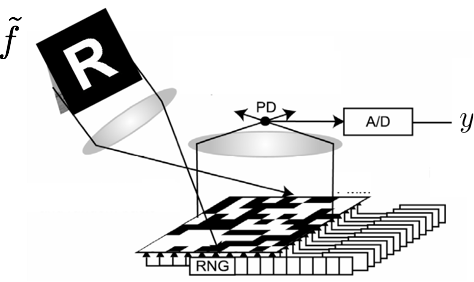
\includegraphics[width=.45\linewidth]{cs/single-pixel/single-pixel-schema}&
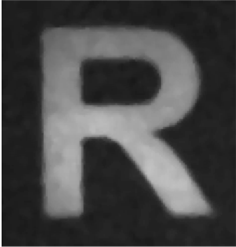
\includegraphics[width=.25\linewidth]{cs/single-pixel/reconstruction-1}&
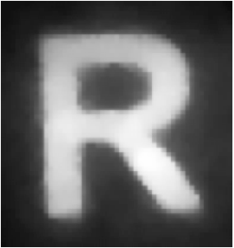
\includegraphics[width=.25\linewidth]{cs/single-pixel/reconstruction-6}\\
Diagram of the device & $f$ & $f^\star$, $P/Q = 6$
\end{tabular}
\caption{Left: diagram of the single-pixel acquisition method.
%
Center: image $f_0 \in \RR^Q$ \guill{ideal} observed in the focal plane of the micro-mirrors.
%
Right: image $f_0^\star = \Psi x^\star$ reconstructed from observation $y \in \RR^P$ with a compression factor $P / Q = 6$ using $\ell^1$-type regularization.
\label{fig-single-pixel}}
\end{figure}


%%%%%%%%%%%%%%%%%%%%%%%%%%%%%%%%%%%%
\subsection{Sparse Recovery}

In order to reconstruct an approximation of the (unknown) image $f_0$, following Section~\ref{sec-sparse-ip}, we assume it is sparse in some dictionary $\Psi$. Denoting $A \eqdef \Psi \Phi \in \RR^{P \times N}$, this leads us to consider the usual $\ell^1$ regularized poblem~\eqref{eq-lasso-lagr-ip}
\eql{\label{eq-lasso-lagr-ip-cs}\tag{$\Pp_\la(y)$}
	x_\la \in \uargmin{x \in \RR^N} \frac{1}{2\la} \norm{y-Ax}^2 + \norm{x}_1, 
} 
so that the reconstructed image is $f_\la = \Psi x_\la$. We also sometimes consider the constraint problem
\eql{\label{eq-lasso-lagr-constr-cs}\tag{$\Pp^\epsilon(y)$}
	x_\epsilon \in \uargmin{\norm{Ax-y} \leq \epsilon} \norm{x}_1, 
} 
where, for the sake of simplicity, we set $\epsilon=\norm{w}$ (which we assume is known). From a mathematical point of view, these problem are equivalent in the sense that there exists a bijection between $\la$ and $\epsilon$ which links it solution. But in practice, this bijection is not explicitly known and depends on $y$.  

Here, it is important to remember that $A$ is drawn from a random matrix ensemble. For an arbitrary $\Psi$, it is hard to analyze this random distribution. If $\Psi$ is orthogonal, and the distribution of the columns of $\Phi$ are invariant by rotation (which is the case if the entries are i.i.d. Gaussian), then $A$ has the same distribution as $\Phi$. In the following, we thus directly models the distribution of $A$ and assumes it has some nice property (typically it is close to being Gaussian i.i.d.). 

%%%%%%%%%%%%%%%%%%%%%%%%%%%%%%%%%%%%
%%%%%%%%%%%%%%%%%%%%%%%%%%%%%%%%%%%%
%%%%%%%%%%%%%%%%%%%%%%%%%%%%%%%%%%%%
\section{Dual Certificate Theory and Non-Uniform Guarantees}
\label{sec-cs-certif}

%%%%%%%%%%%%%%%%%%%%%%%%%%%%%%%%%%%%
\subsection{Random Projection of Polytopes}

When there is no noise, $w=0$ a way to tackle the problem is to use the caracterization of solutions of $(\Pp^0(Ax_0))=(\Pp_0(Ax_0))$ given in Section~\ref{sec-polytope-proj}. According to Proposition~\ref{prop-polytope-proj}, identifiable vectors with sparsity $\norm{x_0}_0=s$ corresponds to $s$-dimensional faces of the $\ell^1$ balls $B_1$ which are mapped to face of the projected polytope $AB_1$. This leads to a combinatorial problems to count the number of face of random polytope. Donoho and Tanner were able to perform a sharp analysis of this problem. They showed the existence of two regimes, using two functions $C_A, C_M$ so that, with high probability (i.e. a probability converging exponentially fast to $1$ with $(n,p)$) on the matrix $A$
\begin{rs}
	\item All $x_0$ so that $\norm{x_0}_0 \leq C_A(P/N)P$ are identifiable.
	\item Most $x_0$ so that $\norm{x_0}_0 \leq C_M(P/N)P$ are identifiable.
\end{rs}
For instance, they show that $C_A(1/4)=0.065$ and $C_M(1/4)=0.25$. Figure~\ref{fig-phase-trans} illustrates numerically these two phase transitions. 
%
This analysis can be shown to be sharp in high dimension, i.e. when $\norm{x_0}_0 > C_M(P/N)P$, then $x_0$ is not identifiable with high probability (this corresponds to a phase transition phenomena). 
%
For large dimensions $(N,P)$, the scaling given by $C_M$ describe very well what one observe in practice. For $P=N/4$ (compression of a factor $4$), one retrieve in practice all vector with sparsity smaller than $P/N$. 
%
The function $C_M$ can be computed numerically, and it can be shown to have a logarithmic grows $C_M(r) \sim \log(r)$ for small $r$. This suggests that for high compression regime, one recovers with $\ell^1$ minimization almost all vector with a sparsity $\norm{x_0}_0$ proportional (up to log factor) to the number of measurements $P$. 


%%%%%%%%%%%%%%%%%%%%%%%%%%%%%%%%%%%%
\subsection{Random Matrices}
\label{sec-random-matrix}

The analysis of the performance $\ell^1$ minimization to solve compressed sensing problem is made possible because of the very precise understanding of the distribution of the singular values of certain random ensemble let us illustrate this in the Gaussian case, which is the simplest, and is very illustrative. 

An important part of the recovery proof relies on controlling the correlation matrix $A_I^*A_I$ of selected columns, and even more importantly, its inverse $(A_I A_I)^{-1}$. These random matrices are called Wishart matrices and inverse Wishart matrices. Such a matrix $B=A_I$ is of size $(P,s)$ and is also drawn from the Gaussian ensemble. 
%
Fixing $s$ and letting $P \rightarrow +\infty$, one has thanks to the low of large numbers $B^*B \rightarrow \Id_s$ almost surely. This is however not a very realistic setting, since in general, one hope to have $s$ almost equal, up to log factor, to $P$.

%%%
\paragraph{Linear growth $P = s/\be$. }

A quite extreme setting is when $s$ grows proportionally to $P$, and impose $s/P = \be$. 
%
In this case, the eigenvalues of $B^*B$ are, for large $p$, essentially contained in the interval $[\la_-,\la_+]$
where $\la_\pm=(1 \pm \sqrt{\be})^2$, $\be \eqdef s/p$, in the sense that the probability distribution of eigenvalues converges (in the weak sense of measures) toward the Marcenko-Pastur law
\eq{
	\foralls (u,v) \in \RR_+^2, \quad
		\PP( \text{eig}(B^\top B) \in [u,v] ) \overset{p \rightarrow +\infty}{\longrightarrow} \int_u^v f_\be(\la) \d \la
}
where one fix the ratio $\be=s/P$, and the Marcenko-Pastur law is
\eq{
	f_\be(\la) \eqdef \frac{1}{2\pi\be \la} \sqrt{ (\la-\la_-)_+(\la_+-\la) } 1_{[\la_-,\la_+]}(\la).
}
Figure~\eqref{fig-marcenko-pastur} illustrates this convergence. 

\begin{figure}
\centering
%%
\begin{tabular}{@{}c@{\hspace{5mm}}c@{}}
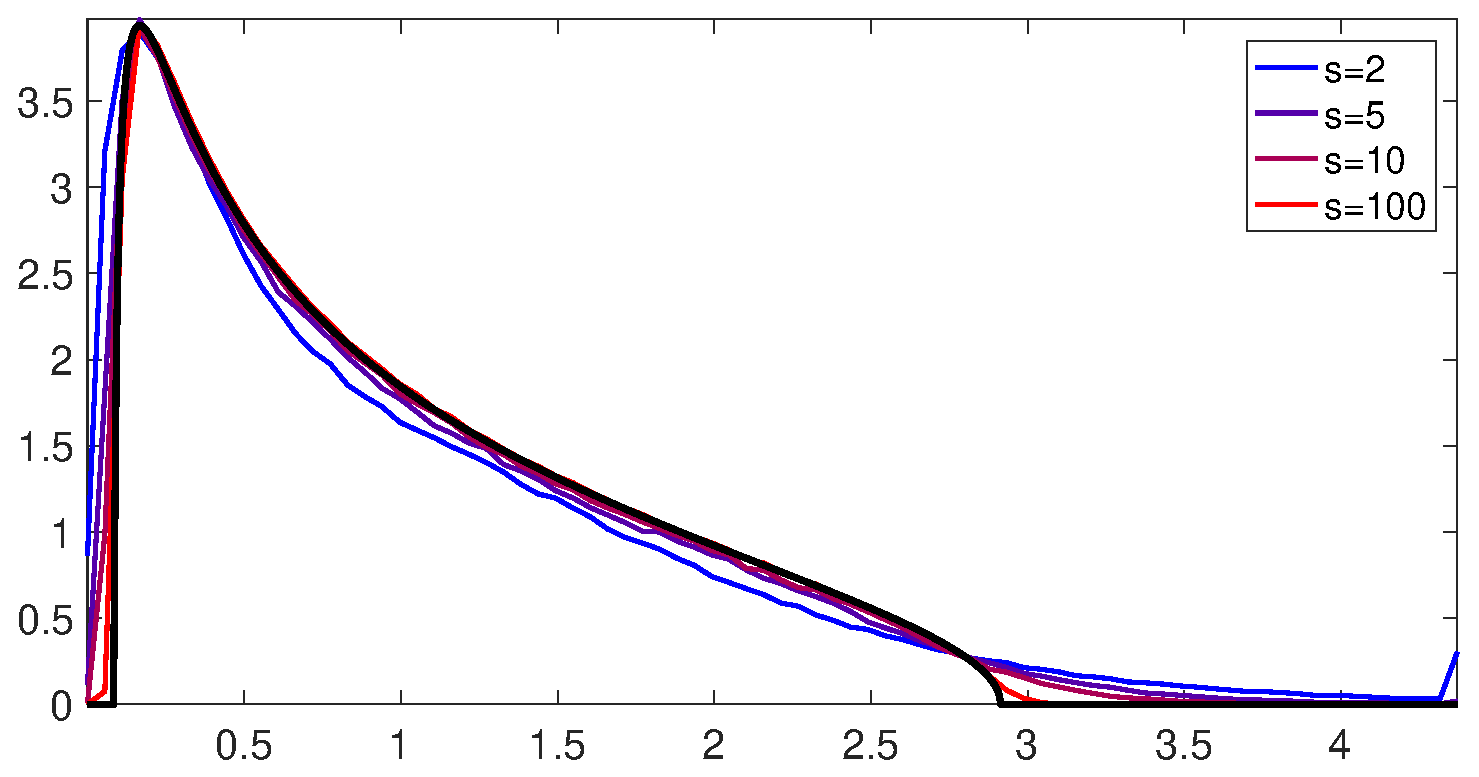
\includegraphics[width=.4\linewidth]{cs/marcenko-pastur/marcenko-pastur-2}&
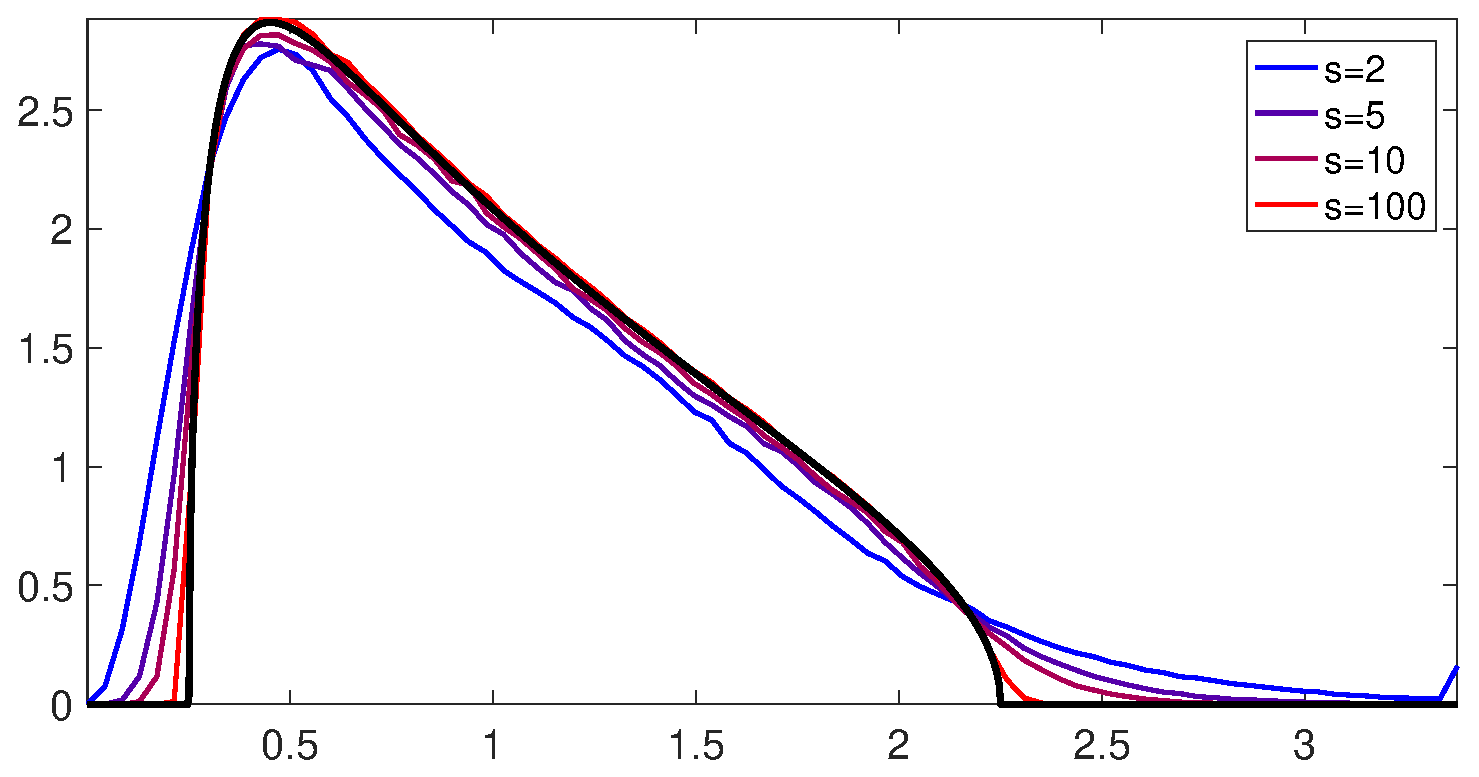
\includegraphics[width=.4\linewidth]{cs/marcenko-pastur/marcenko-pastur-4}\\
$\be=1/2$ & $\be=1/4$ \\
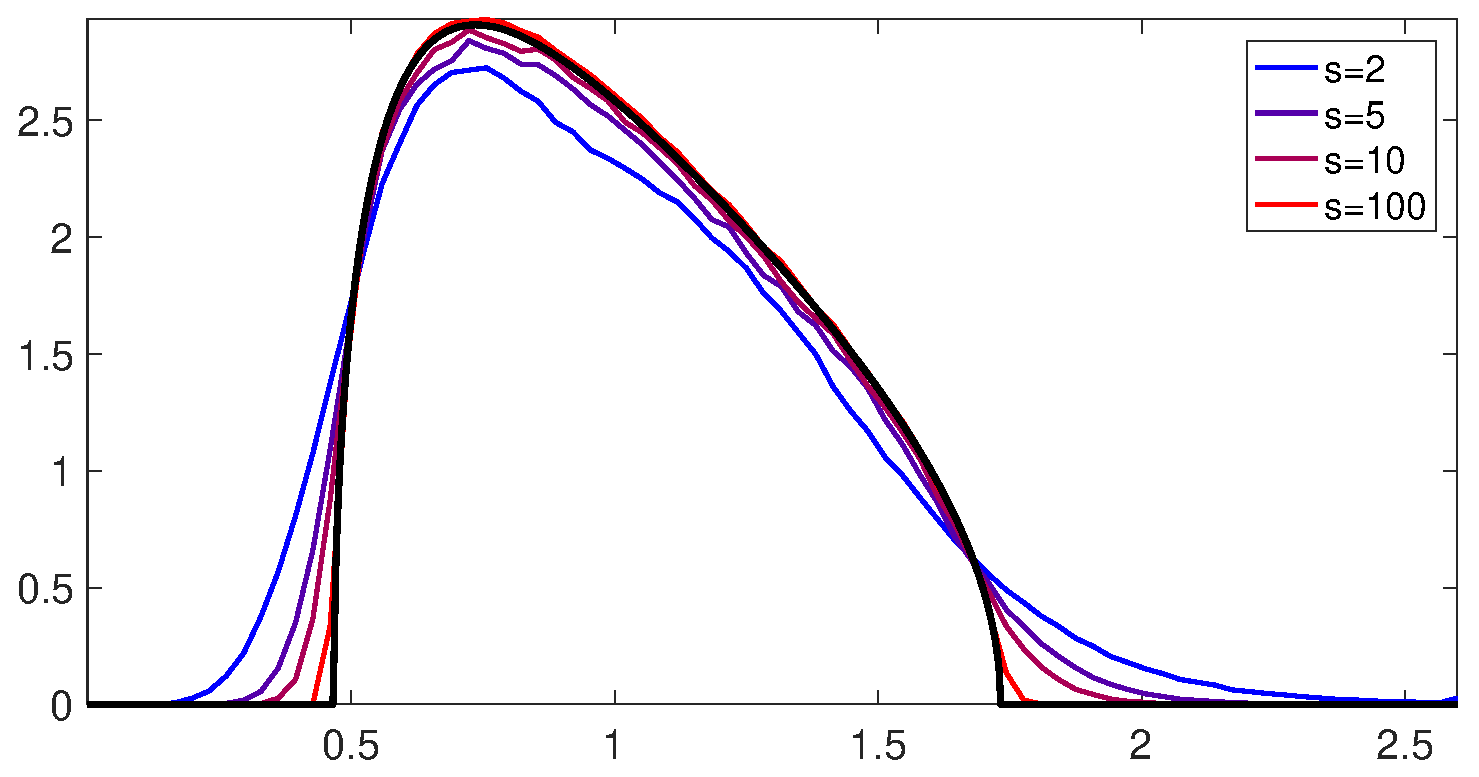
\includegraphics[width=.4\linewidth]{cs/marcenko-pastur/marcenko-pastur-10}&
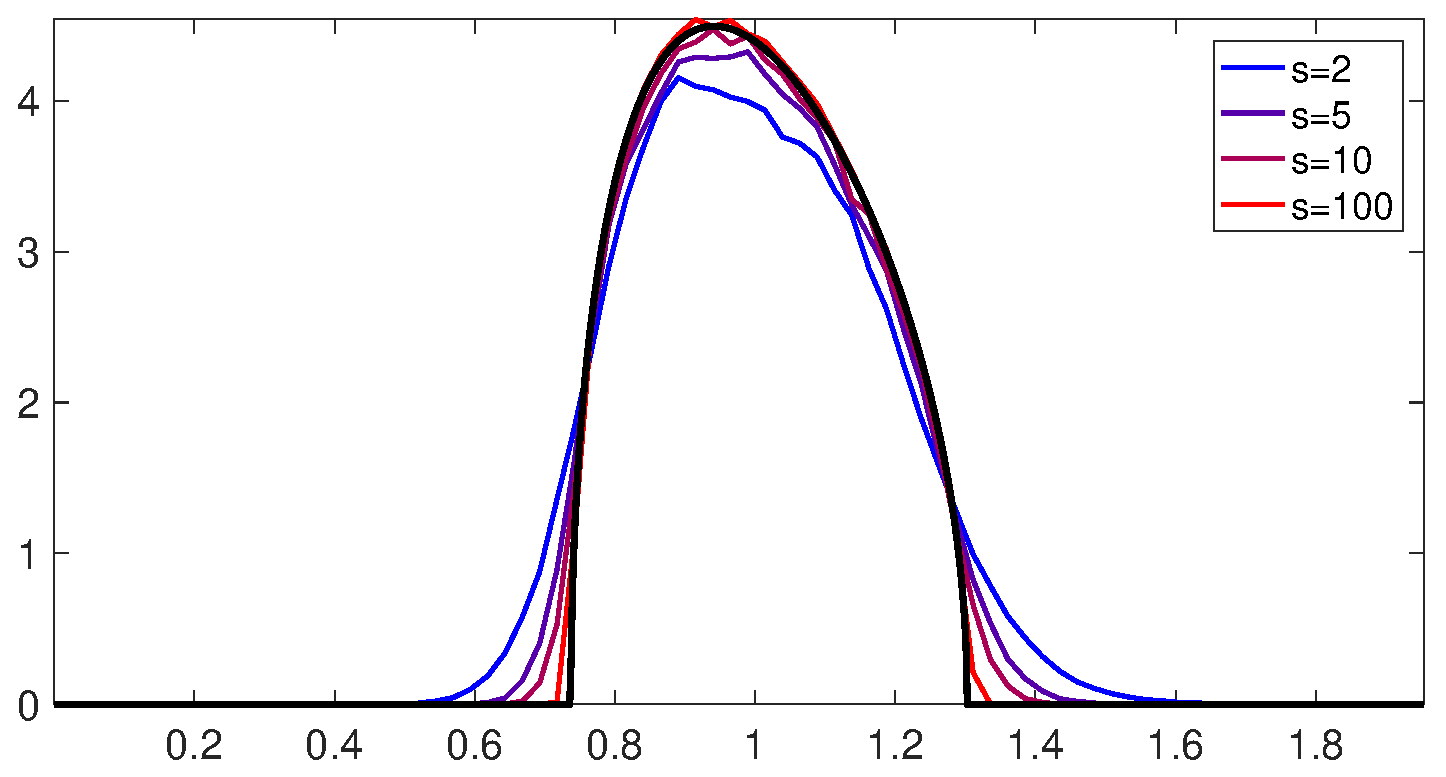
\includegraphics[width=.4\linewidth]{cs/marcenko-pastur/marcenko-pastur-50}\\
$\be=1/10$ & $\be=1/50$ 
\end{tabular}
%%
\caption{\label{fig-marcenko-pastur}
Illustration of the convergence toward the Marcenko-Pastur law.
}
\end{figure}



\begin{figure}
\centering
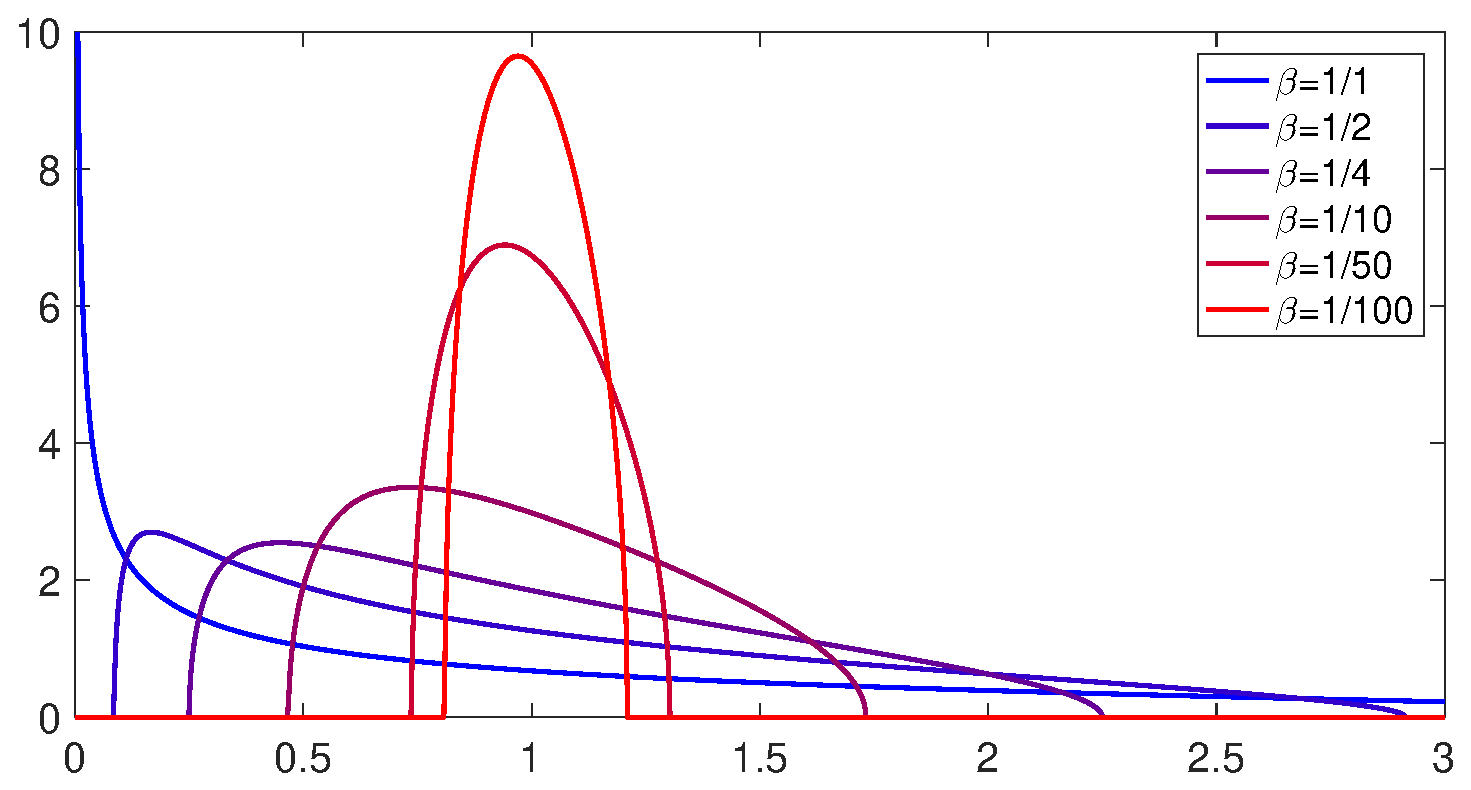
\includegraphics[width=.5\linewidth]{cs/marcenko-pastur/mp-laws.eps}
%%
\caption{\label{fig-marcenko-pastur}
Display of the Marcenko-Pastur distribution $f_\be$ for various $\be$.
}
\end{figure}


%%%
\paragraph{Super-linear grows $P = s \log(\ldots)$. }

In order to have a better concentration of the singular values of $A_I^* A_I$ around $1$, one needs to have a slightly super-linear growth of $P$ with $s$. In this setting one has that $A_I^* A_I$. In order to derive non-asymptotic (i.e. with explicit constants) results, one can use a celebrated concentration inequality due to Talagrand, which assert that one has a fast concentration of this randomized covariance $A_I^* A_I$ toward its expectation $\Id_s$.
\eql{\label{eq-talagrand}
	\PP\pa{ \norm{ A_I^* A_I - \Id_s }_{\text{op}} \geq t + \sqrt{\frac{s}{P}} } \leq e^{ -\frac{t^2s}{2} }. 
}

%%%%%%%%%%%%%%%%%%%%%%%%%%%%%%%%%%%%
%\subsection{Gaussian Width}

% For Gaussian matrices (or at least rotation invariant distributions).

%%%%%%%%%%%%%%%%%%%%%%%%%%%%%%%%%%%%
\subsection{Dual Certificates}

In order to analyze recovery performance, one can looks not only for $\ell^2$ stability ($\norm{x_\la-x_0} \sim \norm{w}$) but also that $x_\la$ has the same support as $x_0$ when $\norm{w}$ is small. As detailed in Section~\ref{sec-sparsistency}, this requires to  ensure that the pre-certificate $\eta_F$ defined in~\eqref{eq-minnorm-certif} is non-degenerated, i.e.
\eql{\label{eq-cond-fuchs}
	\norm{\eta_F}_\infty \leq 1 
	\qwhereq 
	\eta_F = A^* A_I (A_I^*A_I)^{-1} \sign(x_{0,I}).
}
Figure~\ref{fig-certif-cs} suggests that this should be the case if $P$ is large enough with respect to $\norm{x_0}$. This theorem backup this observation.


%%%%%%
\paragraph{Coherence-based analysis.}

We first perform a crude analysis using the so-called coherence of the matrix $A=(a_j)_{j=1}^N$ where the $a_j \in \RR^P$ are the columns of $A$, which we assume to be normalized $\norm{a_j}=1$
\eql{
	\mu \eqdef = \umax{i \neq j } |\dotp{a_i}{a_j}| = \norm{A^*A-\Id_N}_\infty
}
where $\norm{C}_\infty=\max_{i,j} |C_{i,j}|$.
%
The coherence is $0$ for an orthogonal matrix, and is always smaller than $1$, $\mu \in [0,1]$. 
%
The smaller the coherence, the better conditioned the inverse problem $Ax=y$ is, and the more likely is the certificate $\eta_F$ to be non-degenerate, as shown by the following proposition.

\begin{prop}\label{prop-bound-coh}
	One has, denoting $s=\norm{x_0}_0=|I|$ where $I=\supp(x_0)$, for $\mu < \frac{1}{s-1}$, 
	\eql{\label{eq-coh-bound}
		\norm{\eta_{F,I^c}}_\infty \leq \frac{ s\mu }{ 1-(s-1)\mu }
		\qandq
		\norm{p_F}^2 \leq \frac{s}{1-(s-1)\mu}.
	}
	In particular, if $s < \frac{1}{2}\pa{ 1+\frac{1}{\mu} }$, $\norm{\eta_{F,I^c}}_\infty < 1$ and one can thus apply the 
	recovery Theorem~\ref{thm-support-stable}. 
\end{prop}
\begin{proof}
	We recall that the $\ell^\infty$ operator norm (see Remark~\ref{rem-operator-norm}) is
	\eq{
		\norm{B}_\infty = \umax{i} \sum_j |B_{i,j}|.
	}
	We denote $C=A^*A$. One has
	\eq{
		\norm{A_{I^c}^*A_I}_\infty = \umax{j \in I^c} \sum_{i \in I} C_{i,j} \leq s \mu
		\qandq
		 \norm{  \Id_s - A_I^*A_I }_\infty = \umax{j \in I} \sum_{i \in I, i \neq j} C_{i,j} \leq (s-1) \mu
	}
	One also has 
	\begin{align*}
		\norm{(A_I^*A_I)^{-1}}_\infty &= \norm{( (\Id_s - A_I^*A_I) - \Id_s)^{-1}}_\infty
		= \norm{ \sum_{k \geq 0} (\Id_s - A_I^*A_I)^k }_\infty \\
		&\leq \sum_{k \geq 0} \norm{  \Id_s - A_I^*A_I }_\infty^k \leq \sum_{k \geq 0} ((s-1) \mu)^k = \frac{1}{1 - (s-1)\mu}
	\end{align*}
	which is legit because the matrix series indeed converge since $(s-1)\mu<1$.
	%
	Using these two bounds, one has
	\eq{
		\norm{\eta_{F,I^c}}_\infty = 
		\norm{A_{I^c}^* A_I (A_I^*A_I)^{-1} \sign(x_{0,I})}_\infty
		\leq 
		\norm{A_{I^c}^* A_I}_\infty 
		\norm{(A_I^*A_I)^{-1}}_\infty 
		\norm{\sign(x_{0,I})}_\infty 
		\leq 
		(s \mu) \times \frac{1}{1 - (s-1)\mu} \times 1.
	}
	%
	One has 
	\eq{
		\frac{ s\mu }{ 1-(s-1)\mu } \quad\Longleftrightarrow\quad
		2s\mu < 1+\mu
	}
	which gives the last statement.
	%
	One also has
	\eq{
		\norm{p_F}^2 = \dotp{(A_I^*A_I)^{-1}s_I}{s_I} \leq \norm{(A_I^*A_I)^{-1}}_\infty \norm{s}_1 \leq \frac{s}{1 - (s-1)\mu}
	}
\end{proof}

Note that this proof actually shows that if  $s < \frac{1}{2}\pa{ 1+\frac{1}{\mu} }$, all certificate $\eta_F$ are valid, for any sign pattern $\sign(x_0)$. This actually implies a much stronger stability in the sense that whatever the noise $w$ (which might not be small), the support of $x_\la$ is included (not necessarily equal) in the one of $x_0$.

One can show that one always has
\eql{\label{eq-bound-cohe-mat}
	\mu \geq \sqrt{\frac{N-P}{P(N-1)}}
}
which is equivalent to $1/\sqrt{P}$ for $N \gg P$.
%
For Gaussian matrix $A \in \RR^{P \times N}$, one has for large $(N,P) \rightarrow +\infty$
\eq{
	\mu \sim \sqrt{ \log(PN) / P }
}
which shows that Gaussian matrix are close to being optimal for the bound~\eqref{eq-bound-cohe-mat} if $N \gg P$.
%
Applying Proposition~\ref{prop-bound-coh} thus shows that $\ell^1$ regularization is able to recover with a stable support vector with less than $s \sim O(\sqrt{P})$ (ignoring log terms) non-zero coefficients. In face, we will show now that it does much better and recover a proportional number $s \sim O(P)$. This is because the coherence bound~\eqref{eq-coh-bound} is very pessimistic.

%%%%%%
\paragraph{Randomized analysis of the Fuchs certificate.}

We consider here a class of sufficiently ``random'' matrices. 

\begin{defn}[sub-Gaussian random matrix]
A random matrix $\sqrt{P}�A$ is said to be sub-Gaussian if its entries are independent such that $\EE(A_{i,j})=0$ (zero mean) $\EE(A_{i,j}^2)=1/P$ and 
\eq{\label{eq-sub-gaussian}
	\PP(|\sqrt{P}�A_{i,j}| \geq t) \leq \be e^{-\kappa t^2}. 
}
Note that its entries does not needs to be identically distributed, but the sub-Gaussiannity parameter $(\be,\kappa)$ should not depend on $(i,j)$. 
%
Note also the presence of the normalization factor $\sqrt{P}$, which is here to ensure $\EE(\norm{a_j}^2)=1$ where $a_j$ are the columns of $A$.
\end{defn}

Typical example of sub-Gaussian random matrix are Gaussian or Bernoulli matrices. 


\begin{thm}\label{thm-cs-etaf}
	For a given $x_0 \in \RR^N$, denoting $s=\norm{x_0}_0$, and assuming $A$ is sub-Gaussian, then for for any $0 < \epsilon < 1$ provided that
	\eq{
		P \geq \frac{4c}{1-\de} s \log(2N/\epsilon)
		\qwhereq
		\de^2 \eqdef \frac{C}{4c} \pa{ \frac{7}{\log(2N/\epsilon)}+\frac{2}{s} }
	}
	condition~\eqref{eq-cond-fuchs} holds with probability $1-\epsilon$, 
	so that $x_\la$ has the same support and sign as $x_0$ when $(\norm{w}, \norm{w}/\la)$ is small enough.
	% 
	The constant $C,c$, $C=\frac{2}{3\tilde c}$ where $\tilde c \eqdef \frac{\kappa^2}{4\be+2\kappa}$ only depends on the sub-Gaussianity parameter $(\be,\kappa)$ appearing~\eqref{eq-sub-gaussian}, and for Gaussian or Benoulli matrices, $c=1/2$.
\end{thm}

For a Gaussian matrix, the scaling is that one should have $P \geq (2+\de) s \log(N)$ with a high probability. 

\begin{proof}
	We only give the main insight for the proof. Its crux relies on the fact that $\norm{A_{I^c}^* p_F}_\infty \leq 1$ reads
	\eq{
		\umax{j \notin I} |\dotp{a_j}{p_F}| \leq 1
	}
	where $p_F = A_I^{*+} s_{0,I}$ is \textit{independent} from the vectors $(a_j)_{j \notin I}$ it is correlated against. 
	%
	This allows one to check this condition by first controlling $\norm{p_F}$ and then making as if $p_F$ was a fixed deterministic vector. 
	%
	Noticing 
	\eq{
		\norm{p_F}^2 = \dotp{ A_I (A_I^*A_I)^{-1} s_{0,I} }{ A_I (A_I^*A_I)^{-1} s_{0,I} }
		= \dotp{(A_I^*A_I)^{-1} s_{0,I}}{s_{0,I}}, 
	}
	the heuristic reasoning is that, following what we said in Section~\eqref{sec-random-matrix}, if $P$ grows slightly (logarithmically) faster than $s$, $A_I^*A_I$ is close to $\Id_s$ (see Talagrand inequality�~\eqref{eq-talagrand}), so that 
	\eql{\label{eq-estimate-pf-norm}
		\norm{p_F}^2 \sim \norm{s_{0,I}}^2 = s
	}
	For a \textit{fixed} $p_F$, one has that $\dotp{a_j}{p_F}$ is Gaussian distributed with variance $\norm{p_F}^2/P$, and 
	we use the well known fact (already encountered for denoising using thresholding) that the maximum of $P-s$ such vectors concentrates just below the universal threshold $\norm{p_F}\sqrt{2 \log(N-s)/P}$. Using the estimate~\eqref{eq-estimate-pf-norm}, one sees that $\norm{p_F}_\infty \leq 1$ is implied by $2\log(N)s/P \leq 1$, which gives the sharp scaling $P \geq 2\log(N) s$. 
	
	In order to get robustness to noise, one needs to impose that $\norm{A_{I^c}^* p_F} < 1$, which can be achieve by using a slightly stronger scaling  $P \geq 2(1+\de)\log(N) s$ for a small $\de$.
	
	One can actually make this reasoning very precise, because quite surprisingly, it turns out that $Ps/\norm{p_F}^2$ is actually distributed according to a $\chi^2$ variable with $P-s+1$ degrees of freedom (i.e. the sum of $P-s+1$ squares of Gaussian variables). 
	%
	Indeed, for $s=1$, one immediately sees that $P/\norm{p_F}^2$ is $\chi^2$ with $P$ degrees of freedom. The general case is more involved, and the proof relies on the fact that the isotropy of the distribution implies that $p-P/\norm{p_F}^2$ is the square of the distance between the first column of $A_I$ and the linear space spanned by the other columns (hence $P-s+1$ degrees of freedom).
	%
	Since one has a very good understanding of the clustering of such a $\chi^2$ variable around its means, one can thus show that $\norm{p_F} \leq (1-\de) \sqrt{s}$ with high precision for arbitrary small $\de>0$.
\end{proof}


\begin{figure}
\centering
%%
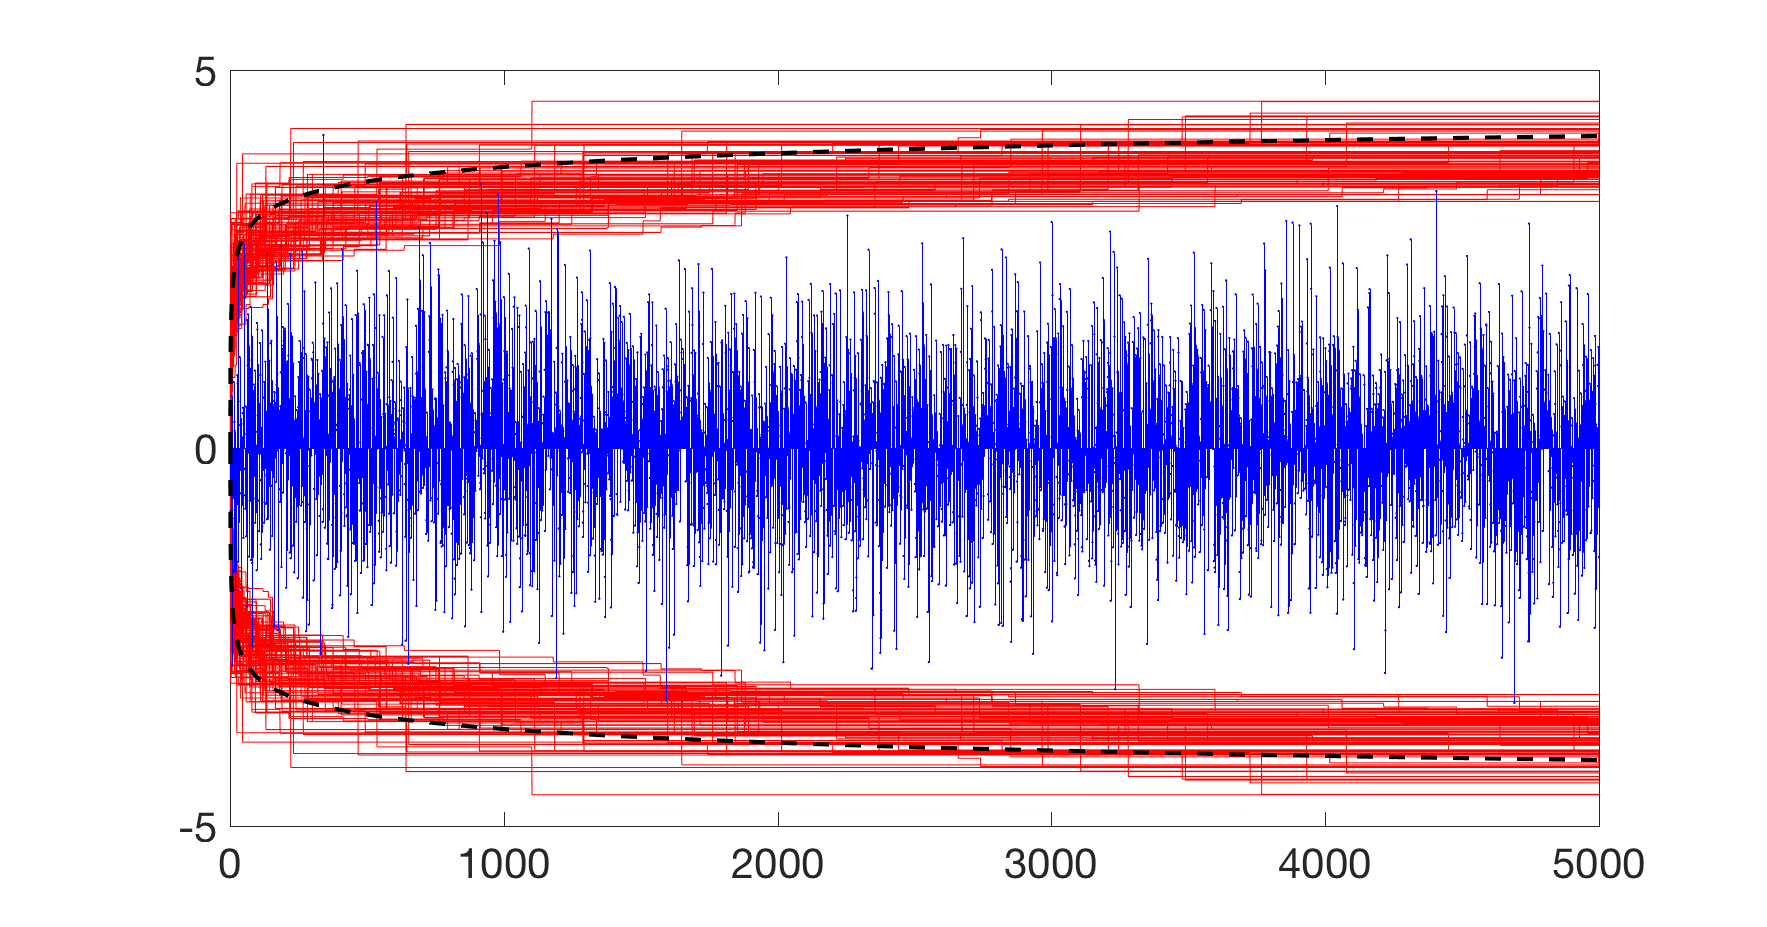
\includegraphics[width=.6\linewidth]{cs/max-gaussian/max-gaussian}
%%
\caption{\label{fig-max-gaussian}
Graphical display of how the maximum of $N$ i.i.d. gaussians concentrates tightly just below the $\sqrt{2\log(N)}$ dashed curve. 
}
\end{figure}
 
For $(N,s) \rightarrow +\infty$, one has $\de \rightarrow 0$, so that informally, the scaling is 
\eql{\label{eq-etaf-gaussiancase}
	P \geq 2s \log(2N/\epsilon).
}
This theorem states a non-uniform recovery guarantee, in the sense that one first choose a vector $x_0$, \text{then} draws the matrix $A$, and the recovery results holds with high probability. This should be contrasted with the RIP theory developed in Section~\ref{sec-rip} which provides stronger uniform guarantees.


\begin{figure}
\centering
%%
\begin{tabular}{@{}c@{}c@{}c@{}}
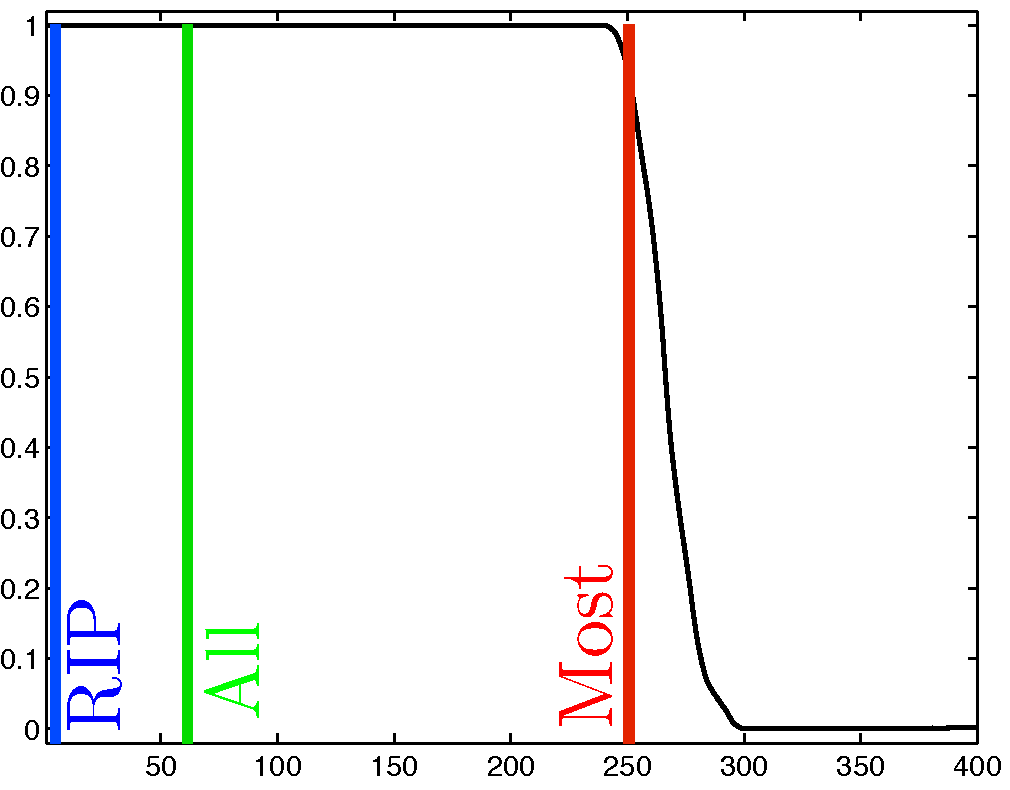
\includegraphics[width=.35\linewidth]{cs/phase/phase-transition-1}&
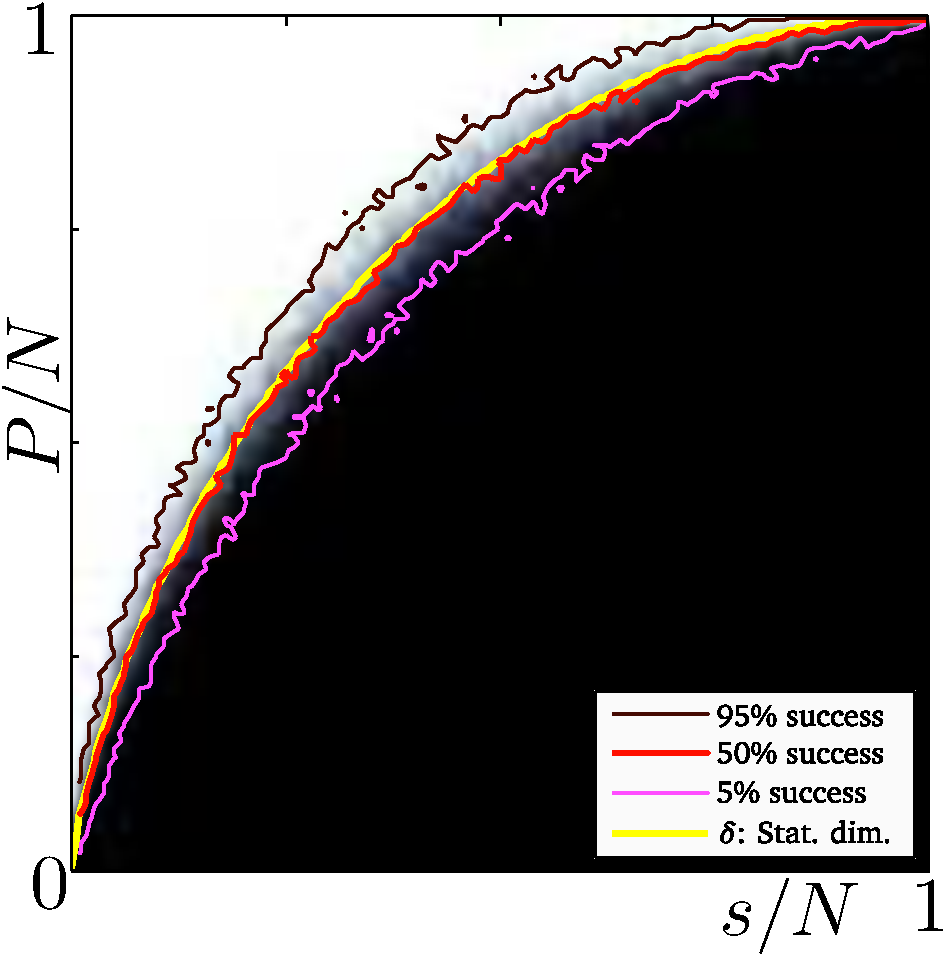
\includegraphics[width=.28\linewidth]{cs/phase/phase-transition-2}&
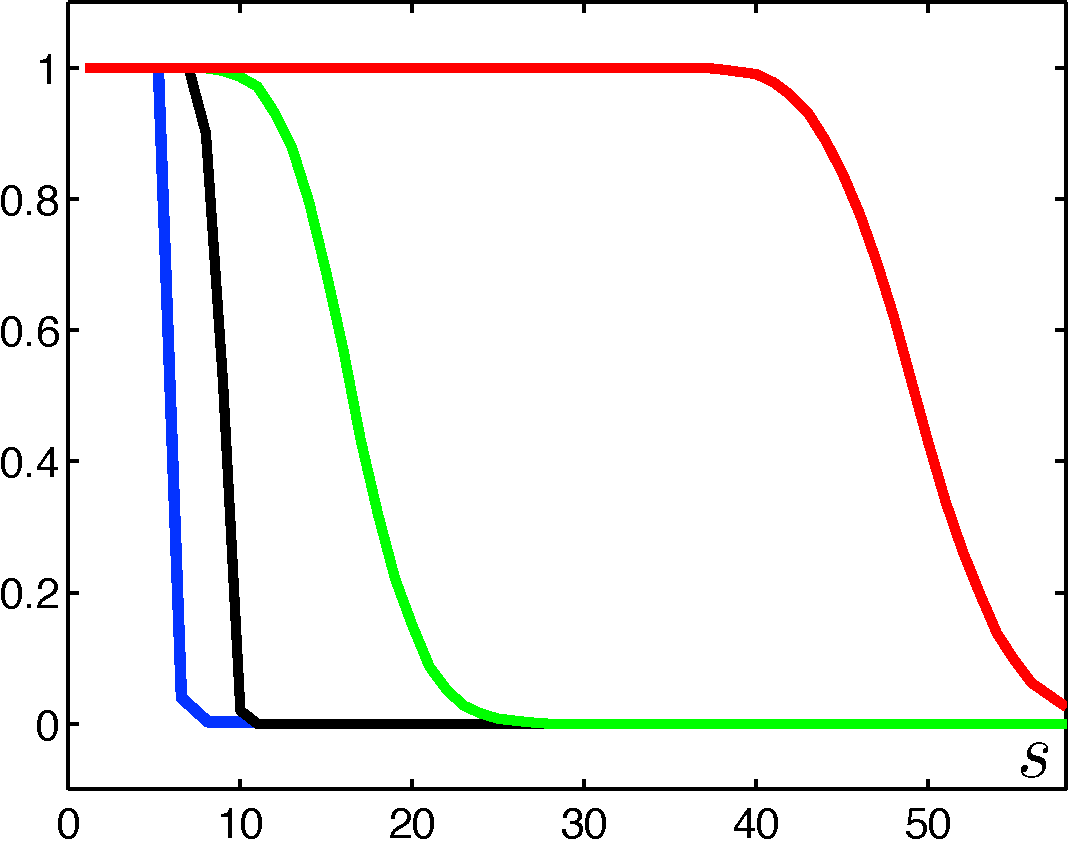
\includegraphics[width=.35\linewidth]{cs/phase/phase-transition-crit}
\end{tabular}
%%
\caption{\label{fig-phase-trans}
Phase transitions. For the figure on the right shows probability as function of sparsity that certain criteria hold true, 
blue: w-ERC,  black: ERC, green $|\eta_F| \leq 1$, red: identifiability. 
}
\end{figure}



%%%%%%%%%%%%%%%%%%%%%%%%%%%%%%%%%%%%
%%%%%%%%%%%%%%%%%%%%%%%%%%%%%%%%%%%%
%%%%%%%%%%%%%%%%%%%%%%%%%%%%%%%%%%%%
\section{RIP Theory for Uniform Guarantees}
\label{sec-rip}

%%%%%%%%%%%%%%%%%%%%%%%%%%%%%%%%%%%%
\subsection{Restricted Isometry Constants}

The Restricted Isometry constant $\de_s$ of a matrix $A \in \RR^{P \times N}$ is defined as
\eql{\label{eq-rip}
	\foralls z \in \RR^N, \quad
	\normz{z} \leq s \qarrq
	(1-\de_{s}) \norm{z}^2 \leq \norm{A z}^2 \leq (1+\de_{s}) \norm{z}^2, 
}
and one usually chose the smallest $\de_s$ so that these relation hold.

A related concept is the $(s,s')$ restricted orthogonality constant $\th_{s,s'}$, which is such that for all $(x,x')$ with $\norm{x}_0 \leq s$, $\norm{x'}_0 \leq s'$ and disjoint support , one has
\eq{
	|\dotp{A x}{A x'}| \leq \th_{s,s'} \norm{x} \norm{x'}
}
The following lemma shows that RI and RO constants are tightly related.

\begin{lem}\label{lemma-rip-roc}
	One has
	\eq{
		\th_{s,s'} \leq \de_{s+s'} \leq \th_{s,s'} + \max(\de_s,\de_{s'}). 
	}
\end{lem}
\begin{proof}
	We prove the first inequality (which is the most important). 
	%
	We prove that if $z$ and $z'$ have disjoints supports and $\norm{z} \leq s$ and $\normz{z'} \leq s$, 
	\eq{
		|\dotp{A z}{A z'}| \leq \de_{2s} \norm{z}\norm{z'}.
	}	
	Using the RIP \eqref{eq-rip} since $z \pm z'$ has support of size $s+s'$ and the fact that $\norm{z \pm z'}^2 = \norm{z}^2 + \norm{z'}^2$, one has
	\eq{
		(1-\de_{s+s'}) \pa{ \norm{z}^2 + \norm{z'}^2 } 
		\leq \norm{A z \pm A z'}^2 \leq
		(1+\de_{s+s'}) \pa{ \norm{z}^2 + \norm{z'}^2 } .
	}
	One thus has using the parallelogram equality 
	\eq{
		|\dotp{A z}{A z'}| =
		\frac{1}{4}
		| \norm{A z + A z'}^2 - \norm{A z - A z'}^2 |
		\leq
		\de_{s+s'} \norm{z}\norm{z'}.
	}
\end{proof}


\begin{figure}
\centering
%%
%\begin{tabular}{@{}c@{\hspace{5mm}}c@{}}
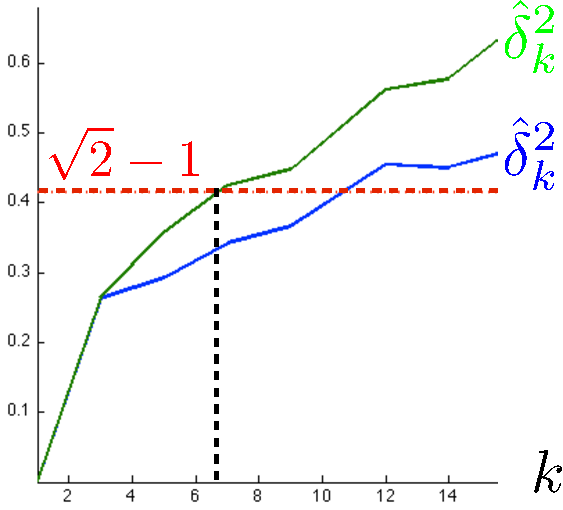
\includegraphics[width=.35\linewidth]{cs/rip-const/delta-k}
%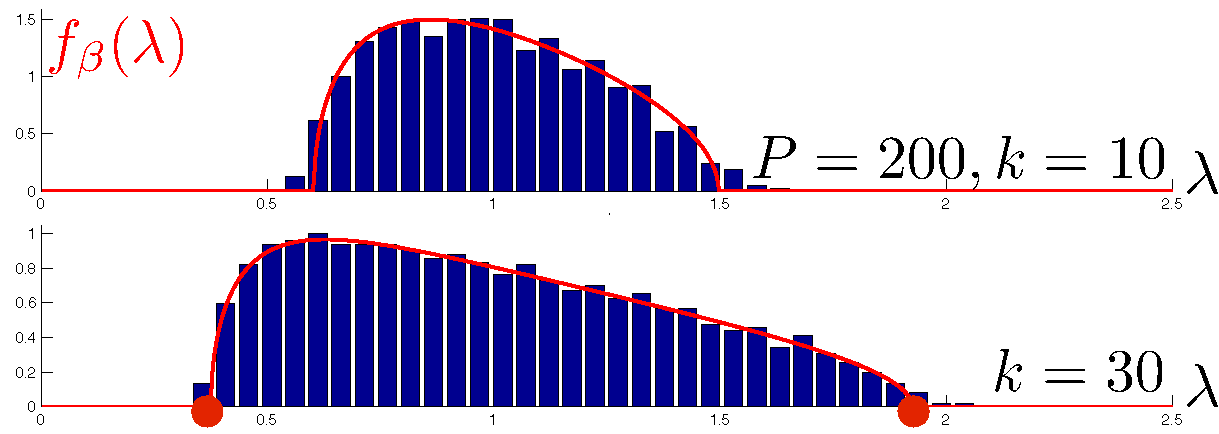
\includegraphics[width=.55\linewidth]{cs/rip-const/eigen-distrib}
%\end{tabular}
%%
\caption{\label{fig-rip-const}
Left: evolution of lower bounds $\hat \de_k$ on the RIP constant. 
% Right: empirical distribution of singular values of Gaussian matrices.
}
\end{figure}

The following theorem states that for a sub-Gaussian random matrix, these RIP constants grow slowly with $s$.
%
Let us stress that, although this is an abuse of notation, here we assume that $A$ is a random matrix, and not a deterministic one as previously considered. 

\begin{thm}\label{thm-rip-random}
	If $A$ is a sub-Gaussian random matrix, then provided
	\eql{
		P \geq C \de^{-2} s \log(eN/s)
	}
	it satisfies $\de_s \leq \de$ with probability $1 - 2e^{ -\de^2 \frac{m}{2C} }$, where $C$ only depends on the sub-Gaussianity parameters appearing in~\eqref{eq-sub-gaussian}.
\end{thm}


We do not prove this Theorem, and simply give the main intuition. 
%
The proof of this theorem relies on results regarding the distribution of the singular values of Gaussian matrices. Indeed, the RIP condition~\eqref{eq-rip} is equivalent to having the bound $\text{eig}( A_I^* A_I ) \subset [1-\de_s,1+\de_s]$ for all Gaussian matrices $A_I$ extracted from $A$. 
%
In the Gaussian case (actually this holds for any random matrix with i.i.d. entries and unit covariance), one has a very good understanding of the distribution of the singular values of covariance matrices $B^*B \in \RR^{s \times s}$ of a Gaussian matrix $B$ of size $(P,s)$, $B \sim \texttt{randn}(P,s)/\sqrt{P}$, as detailed in Section~\ref{sec-random-matrix}.  In particular, using Talagrand concentration inequality~\eqref{eq-talagrand}, one obtains the desired controls over the $\de_s$ constants. 
%
The intuition is that, if we assume that $s/P=\be$ is constant and $P$ is large, then one has that the eigenvalue of $A_I^*A_I$, and for instance its smaller one should be of the order of $2\sqrt{s/P}-s/P$, so that $\de_s$ should be a function of $s/P$, and hence $P$ should scale proportionally to the $s$. The log term comes from the exponential number of such matrix to control, and one need to use a non-asymptotic lower bound in place of the Marcenko-Pastur asymptotic law. 


%%%%%%%%%%%%%%%%%%%%%%%%%%%%%%%%%%%%
\subsection{RIP implies dual certificates}

The following theorem ensures that having small enough restricted isometry constant implies the existence of a valid dual certificates. This means that one can apply Theorem~\ref{thm-linrate-l1}, which in turn ensures that one has a stable recovery of sparse signals.

\begin{thm}\label{thm-rip-dualcertif}
	If $\de_s + \th_{s,s} + \th_{s,2s} < 1$, then for any $x_0$ with $\norm{x_0} \leq s$, there exists $\eta \in \Dd_0(A x_0,x_0)$, i.e. $\eta \in \Im(A^*) \cap \partial\norm{x_0}_1$. More precisely, one has, denoting $I=\supp(x_0)$, $\eta_I = \sign(x_{0,I})$ and
	\eq{
		\norm{\eta_{I^c}}_\infty \leq \frac{\th_{s,s}}{1-\de_s-\de_{s,2s}} < 1
		\qandq
		\norm{p} \leq \frac{\de_{s,s}}{ 1-\de_s-\th_{s,2s} } \frac{\sqrt{s}}{\sqrt{1-\de_s}}. 
	}	  
\end{thm}

Note that thanks to Lemma~\ref{lemma-rip-roc}, condition 
\eq{
	\de_s + \th_{s,s} + \th_{s,2s} \leq \de_s+\de_{2s}+\de_{3s} \leq 3 \de_{3s} 
} 
so that condition $\de_s + \th_{s,s} + \th_{s,2s} < 1$ is implied by $\de_{3s}<1/3$. It is furthermore possible to refine the proof of this theorem to obtain alternative (often much sharper) sufficient condition such as $\de_{2d} \leq \sqrt{2}-1$. 
%
These sufficient conditions involving RI constants are often called ``Restricted Isometry Properties'' (RIP). 
%
As we will illustrate next, however, the constant involved on the sufficient sparsity to guarantee that such uniform RIP conditions holds are large, of the order of a few hundred.

To prove this theorem, it is not enough to directly consider the pre-certificate $\eta_F$ defined in~\eqref{eq-cond-fuchs}. Indeed, using such a certificate leads to slightly suboptimal log-factors in the asymptotic. The proof strategy, developed by Candes and Tao (in ``Decoding with Linear Programming'') consists in iteratively ``improving'' this certificate by removing a vector interpolating the largest $s$ entries outside $I$. 
%
In order to study $\eta_F$ and to perform the improvement, it is crucial the behavior of least square solution of interpolation problems using random matrices.

\begin{lem}\label{lemma-rip-eta}
	We assume $\de_s < 1$.	
	%
	Let $c \in \RR^n$ with $\norm{c}_0 \leq s$ and $\supp(c)=J$. 
	%
	Let $\eta=A^* p$ be the least square solution of $\eta_J=A_J^*p=c_J$, i.e. 
	\eq{
		p \eqdef A_J^{*,+} c_J = A_J (A_J^*A_J)^{-1} c_J
	}
	(note that $A_J$ is full rank because $\de_s<1$). Then, denoting $K \subset J^c$ the $s'$ largest entries in magnitude of $\eta_{J^c}$, one has
	\eq{
		\norm{\eta_{(J \cup K)^c}}_\infty \leq \frac{\th_{s,s'} \norm{c}}{(1-\de_s) \sqrt{s}}
		\qandq
		\norm{\eta_K} \leq \frac{\th_{s,s'} \norm{c}}{1-\de_s}
		\qandq
		\norm{p} \leq \frac{\norm{c}}{\sqrt{1-\de_s}}  
	}
\end{lem}
\begin{proof}
	Since $|J|\leq s$, one has that $\la_{\min}(A_J^*A_J) \geq 1-\de_s$ and hence 
	\eq{
		\norm{(A_JA_J^*)^{-1}} \leq \frac{1}{1-\de_s}
	}
%		\qandq
%		\norm{A_J^{+,*}} = \norm{A_J (A_JA_J^*)^{-1}} \leq \frac{\sqrt{1+\de_s}}{1-\de_s}.
%	}
	One has
	\eq{
		\norm{p}^2 = \dotp{A_J (A_J^*A_J)^{-1} c_J}{A_J (A_J^*A_J)^{-1} c_J}  =
			\dotp{(A_J^*A_J)^{-1} c_J}{c_j} \leq \frac{\norm{c}^2}{ 1-\de_s }.
	}
%	This last inequality shows that $\norm{p} \leq \frac{\sqrt{1+\de_s}}{1-\de_s} \norm{c}$. 
	%
	Let $L$ be any set with $L \cap J = \emptyset$ and $|L| \leq s'$. 
	One has
	\eq{
		\norm{\eta_L}^2 = 
		|\dotp{\eta_L}{\eta_L}| = |\dotp{A_J (A_J^*A_J)^{-1} c_J}{A_L \eta_L}| \leq \th_{s,s'} \norm{(A_J^*A_J)^{-1} c_J} \norm{\eta_L}
			\leq \frac{\th_{s,s'}}{1-\de_s} \norm{c_J} \norm{\eta_L}.
	}
	so that this gives 
	\eql{\label{eq-proof-lemma-rip-eta-1}
		\norm{\eta_L} \leq \frac{\th_{s,s'}}{1-\de_s} \norm{c_J}.
	}
	Let us denote $\bar K = \enscond{ k \in J^c }{ |\eta_k|>T }$ where $T \eqdef \frac{\th_{s,s'}}{(1-\de_s)\sqrt{s'}} \norm{c_J}$. One necessarily has $|\bar K| \leq s'$, otherwise one would have, taking $K \subset \bar K$ the $s'$ largest entries (in fact any $s'$ entries) 
	\eq{
		\norm{\eta_K} > \sqrt{s' T^2} = \frac{\th_{s,s'}}{1-\de_s} \norm{c_J}
	}
	which contradicts~\eqref{eq-proof-lemma-rip-eta-1}. This shows that the entries in $\eta_{J^c}$ after the rank $s'$ are smaller than $T$.
\end{proof}

We can now prove the Theorem~\ref{thm-rip-dualcertif}.

\begin{proof}
	We denote $I_0=\supp(x_0)$. We first consider $\eta_1=\eta_F$, $p_1=p_F$, and we use~\eqref{lemma-rip-eta} with $c_I=\si_I \eqdef \sign(x_{0,I})$, $J=I$, $s'=s$, to control this first pre-certificate. This lemma defines a second set $I_1$ (denoted $K$ in the lemma) which are the $s$ largest entries of $\eta_{1,I_1^c}$, with
	\eq{
		I_0 \cap I_1 = \emptyset, \quad
		|I_1| \leq s, \quad
		\eta_{1,I_0}=s_I, \quad 
		\norm{\eta_{1,(I_0 \cup I_1)^c}}_\infty \leq \frac{\th_{s,s}}{1-\de_s}, \quad
		\norm{\eta_{I_1}} \leq \frac{\th_{s,s} \sqrt{s}}{1-\de_s}, \quad
		\norm{p_1} \leq \frac{\sqrt{s}}{\sqrt{1-\de_s}}. 
	}
	%
	Now we proceed recursively. Having defined the vectors $(\eta_1=A^*p_1,\ldots,\eta_n=A^*p_n)$ with associated sets $(I_1,\ldots,I_n)$, we define $\eta_{n+1}=A^* p_{n+1}$ and $I_{n+1}$ by applying~\eqref{lemma-rip-eta} to $J=I_0 \cup I_n$ with $c=(0_{I_0},\eta_{n,I_n})$ (and thus $(2s,s)$ in place of $(s,s')$), which hence satisfy
	\eq{
		I_{n+1} \cap (I_0 \cup I_{n}) = \emptyset, \quad
		|I_{n+1}| \leq s, \quad
		\eta_{n+1,I_0 \cup I_n} = (0_{I_0},\eta_{n,I_n}), \qandq
	}
	\eql{\label{eq-proof-rip-dualcertif-1}
		\norm{\eta_{n+1,(I_0 \cup I_n \cup I_{n+1})^c}}_\infty \leq \frac{\th_{s,s}}{1-\de_s} 
			Q^n, \quad
		\norm{\eta_{n+1,I_{n+1}}} \leq \frac{\th_{s,s} \sqrt{s}}{1-\de_s} Q^n,
	}
	where we denoted $Q \eqdef \frac{\th_{s,2s}}{1-\de_s}$, 
	and we have
	\eq{
		\norm{p_{n+1}} \leq \frac{ \norm{\eta_{n,I_n}} }{ \sqrt{1-\de_s} } 
		\leq
			\frac{1}{\sqrt{1-\de_s}} \frac{\th_{s,s} \sqrt{s}}{1-\de_s} Q^{n-1}.	
	} 
	%
	Since $\de_s+\th_{s,s} < 1$, one has that $Q<1$, and thus setting
	\eq{
		p = \sum_{n=1}^{+\infty} (-1)^{n-1} p_n
		\qandq
		\eta = A^*p
	}
	defines a convergent series.
	%
	By construction, since $\eta_{1,I}=\si$ and $\eta_{n,I}=0$ for $n>1$, one has $\eta_I=\si_I$, thus this vector interpolates the sign vector $\si$.
	%
	Now consider $j \in I^c$ and define $E_j \eqdef \enscond{n \geq 1}{ j \in I_n } = \{n_1 \leq n_2 \leq n_3 \leq \ldots\}$. Since $I_n \cap I_{n+1} = \emptyset$, necessary $n_{k+1} \geq n_k+2$ ($j$ cannot belong to two consecutive $I_n$). 
	%
	Furthermore, if $n \in E_j \Leftrightarrow j \in I_n$, then by construction
	\eq{
		\eta_{n,j} = \eta_{n+1,j}
	}
	so that these two consecutive terms cancels out in the sum defining $\eta$ \todo{make a drawing}, which in turn can thus be written in the form
	\eq{
		\eta = \sum_{n \in H} (-1)^{n-1} \eta_n.
	}
	The index set $H$ is composed of $n \notin E_j$ such that $n-1 \notin E_j$ (because otherwise one could cancel $\eta_n$ from the sum). 
	%
	So this means that for $n \in H$, one has $j \notin (I_0 \cup I_n \cup I_{n+1})$, thus applying the property~\eqref{eq-proof-rip-dualcertif-1}, one has
	\eq{
		\foralls n \in H, \quad |\eta_{j,n}| \leq \frac{\th_{s,s}}{1-\de_s} 
			Q^{n-1}, 
	}
	so that 
	\eq{
		|\eta_j| \leq \sum_{n \in H} |\eta_{j,n}| \leq \sum_{n=1}^{+\infty} \frac{\th_{s,s}}{1-\de_s}  Q^{n-1}
		= \frac{\th_{s,s}}{1-\de_s} \frac{1}{1- \th_{s,2s}(1-\de_s)^{-1} }
		= \frac{\th_{s,s}}{ 1-\de_s-\th_{s,2s} }.
	}
	Note that one also has the bound
	\eq{
		\norm{p} \leq \sum_n \norm{p_n} \leq \sum_n \frac{1}{\sqrt{1-\de_s}} \frac{\th_{s,s} \sqrt{s}}{1-\de_s} Q^{n-1}
		= \frac{\de_{s,s}}{ 1-\de_s-\th_{s,2s} } \frac{\sqrt{s}}{\sqrt{1-\de_s}}.
		% O( \sum_n Q^n \sqrt{s} ) = O(\sqrt{s}).
	}
\end{proof}

%%%%%%%%%%%%%%%%%%%%%%%%%%%%%%%%%%%%
\subsection{RIP implies stable recovery}


Putting together Theorems~\ref{thm-rip-random}�and~\ref{thm-rip}, and using the general inverse prolem stability theorem~\ref{}, one obtains the following recovery guarantee.

\begin{thm}\label{thm-rip-final}
	If $A$ is a sub-Gaussian random matrix, then there exists constants $(C,C')$ such that provided 
	\eql{\label{eq-thm-rip-final}
		P \geq C s \log(N/s)		
	}
	with probability $1 - 2e^{ -C' P}$ on the draw of $A$, one has that for every $s$-sparse signal $x_0$, 
	\eq{
		\norm{x_\la-x_0} = O(\norm{w})
	}
	where $x_\la$ is the unique solution of~\eqref{eq-lasso-lagr-ip} with measurements $y=A x_0 + w$ when choosing $\la \sim \norm{w}$.
	%
%	In particular, if $\norm{w}=0$ and $x_0$ is $s$-sparse, setting $\la=0$, one has $x^\star=x_0$.
\end{thm}

It is possible to extend this theorem when $x_0$ is not exactly $s$-sparse but only approximately. Defining $x_{0,s}$ the best $s$-term approximation, the easiest way to go is to write $y=A x_{0,s}+\tilde w$ where $\tilde w=w+A(x_0-x_{0,s})$ and applying the previous result to obtain
\eq{
	\norm{x_\la-x_{0,s}} = O(\norm{w} + \norm{A}\norm{x_0-x_{0,s}}). 
}
It is possible to obtain better scaling in term of the non-linear approximation error $\norm{x_0-x_{0,s}}$ by doing a more careful proof.


This theorem provides a uniform recovery guarantee, in the sense that it means
\eq{
	\PP( \foralls s-\text{sparse } x_0, x^\star=x_0 ) \text{ goes fast to 1 when } P \rightarrow +\infty. 
}
In contrast, theorem~\ref{thm-cs-etaf} proves a weaker non-uniform guarantee, in the sense that it means
\eq{
	\foralls s-\text{sparse } x_0,  \PP( x^\star=x_0 ) \text{ goes fast to 1 when } P \rightarrow +\infty. 
}

The recovery performance analysis based on RIP constants proves a better scaling in term of log-factors. This is because the analysis using $\eta_F$ does not only imply stable recovery, it also provides stability of the support (sparsistency). Note however that the constants involved in the RIP analysis are very large (of the order of a few hundreds, as highlighted by Figure~\ref{fig-rip-const}, left, and by Figure~\ref{fig-phase-trans}, right), while the constant appearing in~\eqref{eq-etaf-gaussiancase} are small and known to be sharp.

Also, one can show that having small enough RIP constant implies the existence of a valid dual certificate (but this certificate is not necessarily $\eta_F$).






%%%%%%%%%%%%%%%%%%%%%%%%%%%%%%%%%%%%%%%%%%%%%%%%
\subsection{Fourier sampling RIP}

A practical issue is that doing hardware implementing random operators $A$ is very difficult, specially if this operator is ``fully'' random, i.e. if its entries are i.i.d. A more practical option is to use structured sampling operator, which are in some sense ``less random''. A possibility is to consider a random sub-sampling of orthogonal projection of the signal in some ortho-basis $\Xi = (\xi_\om)_{\om=1}^N$ of $\RR^N$, so that
\eql{\label{eq-random-subsample}
	A x \eqdef ( \dotp{x}{\xi_\om} )_{\om \in \Om} \in \RR^P
}  
where $\Om \subset \{1,\ldots,N\}$ is drawn uniformly at random among all sets of size $P$.
%
The following theorem ensure that such an operator satisfies the RIP properties for large $s$ (proportional to $P$ up to log factors) is the atomes $\phi_\om$ are ``spread enough'', i.e. have a small magnitude, as measured by
\eq{
	\rho(\Xi) \eqdef \sqrt{N} \umax{1 \leq \om \leq N} \norm{\xi_\om}_\infty.
}

\begin{thm}[Rudelson-Vershinyn]\label{thm-cs-subsample}
	For any $0<c<1$, there exists $C$, such that provided that 
	\eql{\label{eq-scaling-cs-subsample}
		P \geq C \rho(\Xi)^2 s \log(N)^4
	}
	with high probability on $\Om$, then $A$ defined as in~\eqref{eq-random-subsample} satisfies $\de_{2s} \leq c$.
\end{thm}

One always has $1 \leq \rho(\Xi)^2 \leq N$.
%
The worse case is $\xi_\om$ to be Sirac atoms (i.e. $\Xi=\Id_N$), having $\rho(\Xi)^2=N$, in which case $P$ needs to be as large as $N$. 
%
In sharp contrast, optimal sampling bases are for instance Fourier atoms $\xi_\om = (e^{\frac{2\imath\pi}{N}\om n} )_{n=1}^N \in \CC^N$, for which $\rho(\Xi)=1$ (it is also possible to consider a Hadamard basis for instance). In this case, up to log-factors, the scaling~\eqref{eq-scaling-cs-subsample} is similar to the one for sub-Gaussian matrices~\eqref{eq-thm-rip-final}.

Theorem~\ref{thm-cs-subsample} deals with cases where the data $x_0$ to recover is sparse in the Dirac basis. If the data $f_0$ is sparse in another basis $\Psi=(\psi_m)_{m=1}^N$, one can do a change of variable $x = \Psi^* f$ ($x$ being the coefficients of $f$ in the basis $\Psi$), in which case $\rho(\Xi)$ appearing in~\eqref{eq-scaling-cs-subsample} should be replaced by the mutual coherence between the sampling and the sparsity bases
\eq{
	\rho(\Psi^*\Xi) \eqdef \sqrt{N} \umax{1 \leq \om,m \leq N} |\dotp{\psi_m}{\xi_\om}|.
}
Good recovery performances are thus reached by (sampling,sparsity) pairs which are incoherent. The (Fourier,Dirac) pair is maximally incoherent. In contrast, Wavelet and Fourier are highly coherent. There exists explicit construction of ``noiselets'' bases which are almost maximally incoherent with wavelets. 
%
Note however that in contrast to Gaussian matrices, these structured measurement matrices are not universal, in the sense that there compressed sensing recovery performances depend on the sparsity basis $\Psi$ which is used. 

